\documentclass[12pt]{article}
\usepackage{graphicx}

\title{
Bryan Petzinger \\
Computer Vision \\
HW3 \\
}
\maketitle

\begin{document}

\section{Writeup}
This program is essentially two parts, the first applies Laws texture engergy measures to an image (represented by 2d array of gray tones) and returns the result in the form of a 2d image with 9dimensional vectors as pixels. The 9d vectors are the result of applying each of the 9 final energy maps to the image. The second part of the program performs segmentation via the K-mean clustering algorithm on the 9d vector image obtained from the previous step. \\

When preprocessing and applying the masks to the image in the first step, I handled the boundary cases (where there are not enough neighboring pixels on one or more sides) by ignoring neighbors that don't exist. This is different than the method suggested in class (duplicating the image to create those neighbors) and results in some noise around the border of the image, but the final result looks ok so I left it as is. \\

Overall I think the algorithms were fairly straightforward, I had discussed the implementation before attempting it with some other students so I had a good idea of how to approach the various parts. I had some minor issues with the segmentation part as I was not correctly calculating and assigning the new mean for each cluster initially, but I was able to figure it out after some debugging. One thing I did that helped a lot was create a method for displaying the masked/filtered images as a buffered image so I could visually error check each part of the process.


\begin{figure}[htb]
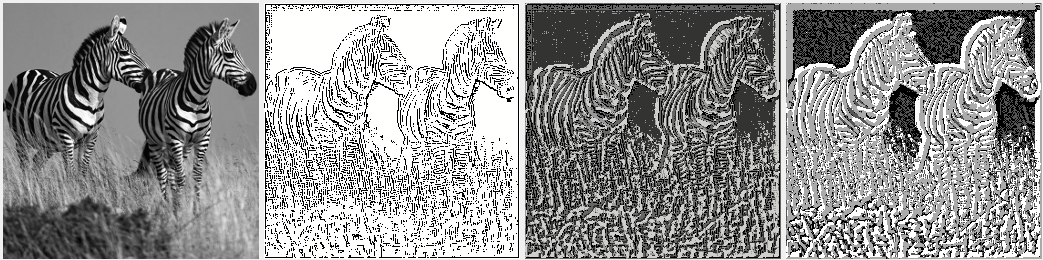
\includegraphics[scale=.5]{result.PNG}
\caption{Results - original, 4 means, 5 means, 6 means}
\end{figure}

\end{document} 
